\setcounter{section}{0}%更改chapter的计数器值
%\numberwithin{equation}{chapter}%公式计数器从属于节计数器
\numberwithin{equation}{section}%公式计数器从属于节计数器
\numberwithin{figure}{section}%图计数器从属于节计数器
\setcounter{chapter}{4}

%\chapter{\texorpdfstring{弦的S矩阵}{5 The string S-matrix}}
\chapter{弦的S矩阵}
在第3章,我们将S矩阵写为带有顶点算符的二维紧致平面上的路径积分,在本章我们会将这一路径积分约化至规范固定形式.
%\section{\texorpdfstring{圆和环面}{5.1 The circle and the torus}}
\section{圆和环面}

我们将一个规范切片,就像图3.7那样等同为从每个(diff $\times $ Weyl) 等价类中一个构型的选择. 定域地,我们通过固定度规实现这一点. 但整体上在度规空间与世界面规范群之间存在一个微小的错配.\\
又一次,点粒子是一个很好的例证. 我们希望计算Euclidean路径积分
\begin{equation}
\int[d e d X] \exp \left[-\frac{1}{2} \int d \tau\left(e^{-1} \dot{X}^{\mu} \dot{X}_{\mu}+e m^{2}\right)\right]
\end{equation}
考察在时空中形成闭合圈的路径,所以拓扑是圆,参量 $\tau$ 可以在0,1之间取值,其中端点是等价的. 即 $X^{\mu}(\tau)$与$e(\tau)$ 在 $0 \leq \tau \leq 1$上有周期性. 四元量 $e(\tau)$ 有一个分量,并存在定域对称性,将四元量完全确定下来. 四元量变换为$e^{\prime} d \tau^{\prime}=e d \tau $ ,因而规范选择给出$\tau^{\prime}(\tau)$的微分方程
\begin{equation}
\frac{\partial \tau^{\prime}}{\partial \tau}=e(\tau)
\end{equation}
对其积分,边界条件 $\tau^{\prime}(0)=0$ 决定了
\begin{equation}
	\tau^{\prime}(\tau)=\int_{0}^{\tau} d \tau^{\prime \prime} e\left(\tau^{\prime \prime}\right)
\end{equation}
问题是,一般情况 $\tau^{\prime}(1) \neq 1$, 所以周期性不被保护. 事实上
\begin{equation}
	\tau^{\prime}(1)=\int_{0}^{1} d \tau e(\tau)=l
\end{equation}
是圆的不变长度. 所以我们不能令 $e^{\prime}=1$ 的同时保持坐标区域不变. 我们可以保持坐标区域不变,令$e^{\prime}$为常数值 $e^{\prime}=l$, 或令 $e^{\prime}=1$ 而让坐标区域变化:
\begin{subequations}
\begin{equation}
e^{\prime}=l, \quad 0 \leq \tau \leq 1
\end{equation}
or
\begin{equation}
e^{\prime}=1, \quad 0 \leq \tau \leq l
\end{equation}
\end{subequations}
无论在哪种情况,在固定规范不变性后,我们留下了对 $l$的普遍积分. 换句话说,不是圆上所有四元基等价. 存在不等价四元基的一个单参量族,由 $l$参量化.\\
(5.1.5) 的两个描述在弦中均有类比. 实际上,我们将用类似 (5.1.5a)的描述来定义路径积分, 其中场是固定坐标区域上的函数,然后转化到类似 (5.1 .5b) 的描述中,其中度规是固定的,而模在坐标范围内被编码.\\
存在与规范固定相关的第二个困难. 条件$e=constant$ 被刚性平移保护
\begin{equation}
	\tau \rightarrow \tau+v \bmod 1
\end{equation}
即在圆上,我们无法说原点在哪. 因而,固定度规留下一小部分非固定的定域对称性,所以在两个方向上存在错误匹配. 度规与另一个不规范等价以及规范变换不被度规选择所固定.\\
转移到弦,我们取圆环面为例,其中会有相同的困难产生. 从坐标区域开始
\begin{equation}
	0 \leq \sigma^{1} \leq 2 \pi, \quad 0 \leq \sigma^{2} \leq 2 \pi
\end{equation}
其中$X^{\mu}\left(\sigma^{1}, \sigma^{2}\right)$ 和 $g_{a b}\left(\sigma_{1}, \sigma_{2}\right)$ 在两个方向都是周期的. 等价地,我们可以视其为在 $\sigma$ 平面上有点等价
\begin{equation}
	\left(\sigma^{1}, \sigma^{2}\right) \cong\left(\sigma^{1}, \sigma^{2}\right)+2 \pi(m, n)
\end{equation}
 $m$ , $n$为整数.\\
场空间diff $\times$ Weyl 冗余到何种程度? 定理是不可能通过一个保持周期性(5.1 .7)不变的diff $\times$ Weyl变换,将一个一般度规变成单位形式,但能够将其变为
\begin{equation}
	d s^{2}=\left|d \sigma^{1}+\tau d \sigma^{2}\right|^{2}
\end{equation}
其中 $\tau$ 是复常数. 当 $\tau=i$ 时,这是单位度规 $\delta_{a b}$.\\
为了看到这一点,重复3.3节定域讨论中所使用的步骤.  首先,我们可以通过一个满足 $2 \nabla^{2} \omega=R $的Weyl变换,使度规平坦.  通过展开 $\nabla^{2}$的本征模,可以看到在有周期边界条件下,其有唯一解至在$\omega $上加一常数.  在这里重要的是 $\int d^{2} \sigma g^{1 / 2} R$, 即 $4 \pi$ 乘以Euler数, 对于环面为零. 之后到新坐标 $\tilde{\sigma}^{a}$ 的变换,将度规变成单位形式. 然而,就像点粒子情况那样,无法保证这反应了原始的周期性. 相反,现在我们可以有
\begin{equation}
	\tilde{\sigma}^{a} \cong \tilde{\sigma}^{a}+2 \pi\left(m u^{a}+n v^{a}\right)
\end{equation}
其中 $u^{a}$ ,$v^{a} $为一般平移. 通过旋转和缩放坐标系,伴随着保持度规归一化的$\omega$偏移,我们总可以令 $u=(1,0)$. 这留下两个参量, $v$的分量. 定义$w=\tilde{\sigma}^{1}+i \tilde{\sigma}^{2}$, 度规是 $d w d \bar{w}$ 周期性是
\begin{equation}
	w \cong w+2 \pi(m+n \tau)
\end{equation}
其中 $\tau=v^{1}+i v^{2} $ ,环面是$w$ 平面中有周期边界条件的平行四边形,如图(\ref{Fig5.1})所示.

\begin{figure}
	\begin{center}
		%width=0.8\textwidth,bb=0 0 654 368
		%1px=0.75pt
		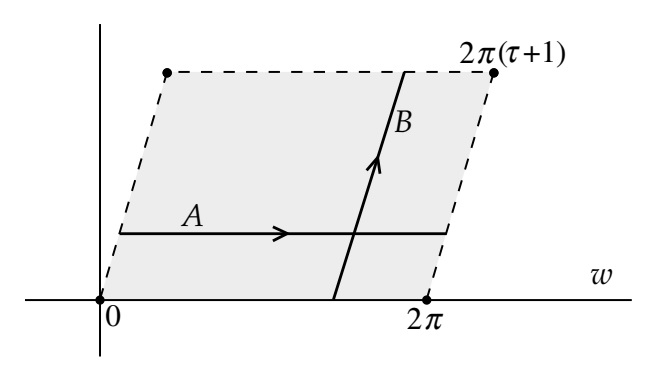
\includegraphics[width=0.5\textwidth,natwidth=490.5,natheight=276]{Fig5.1.jpg}\\
		\caption{Torus with modulus $\tau$, in gauge $d s^{2}=d w d \bar{w}$. The upper and lower edges are identified, as are the right- and left-hand edges. Closed curves $A$ and $B$ are marked for later reference.}\label{Fig5.1}
	\end{center}
\end{figure}


换一种方式,$w=\sigma^{1}+\tau \sigma^{2}$定义用$\sigma^{a}$ . 原始周期性被保留,但度规采取更普遍形式  (5.1 .9) . 对度规的积分退化到对 $\tau $ 实部和虚部的两个积分. 度规 $(5.1 .9)$ 在复共轭下不变,并且对于实的$\tau$简并,所以我们可将注意力集中在  $\operatorname{Im} \tau>0 $,正如圆的情况 $(5.1 .5)$ ,我们可以将这些参量放进度规 (5.1.9) 或周期性(5.1.11)中.参量 $\tau$ 被称为 Teichmüller参量或更普遍的模. 与点粒子不同的是,不存在类似于圆的不变长度那样的 $\tau$ 的简单不变表达式.\\
存在某些额外的冗余,其在点粒子情况没有类似物. 值 $\tau+1$ 生成了与 $\tau$相同的等价集(5.1 .11), 其中替换了 $(m, n) \rightarrow(m-n, n) $ .  $-1 / \tau$ 也是如此. 定义 $w^{\prime}=\tau w$ ,并替换 $(m, n) \rightarrow(n,-m) $ ,重复使用这两个变换
\begin{equation}
	T: \quad \tau^{\prime}=\tau+1, \quad S: \tau^{\prime}=-1 / \tau
\end{equation}
生成了
\begin{equation}
	\tau^{\prime}=\frac{a \tau+b}{c \tau+d}
\end{equation}
其中 $a, b, c, d$是满足$a d-b c=1$的整数.\\
我们也可对其进行如下考虑. 变换
\begin{equation}
	\left[\begin{array}{l}
		\sigma^{1} \\
		\sigma^{2}
	\end{array}\right]=\left[\begin{array}{ll}
		d & b \\
		c & a
	\end{array}\right]\left[\begin{array}{l}
		\sigma^{\prime 1} \\
		\sigma^{\prime 2}
	\end{array}\right]
\end{equation}
使得$\sigma$的度规(5.1 .9) 变成 $\sigma^{\prime}$的相同形式的度规,但模为$\tau^{\prime} $ ,这是环面的微分同胚映射. 由于$a d-b c=1$ ,这是一个一一映射,并保护了周期性 (5.1 .8). 然而,它无法从连续的无穷小变换从恒等变换获得————它是所谓的大坐标变换. 坐标 $\sigma$ 中的曲线A映射到 $\sigma^{\prime}$ 坐标中的曲线沿$A^{\prime}$ 方向伸长a倍,沿 $B^{\prime}$ 方向伸长c倍. 这些大坐标变换构成群 $S L(2, \mathbf{Z})$,  $\tau$ 平面上的群是 $S L(2, \mathbf{Z}) / \mathbf{Z}_{2}=$ $P S L(2, \mathbf{Z})$, 因为如果a, b, c, d符号均不变,$\tau^{\prime}$ 是不变的. 变换 $(5.1 .14)$ 的群称为模群.\\
利用模变换 (5.1.13), 可以证明每个$\tau$ 等价于区域 $F_{0}$中的一个点 ,如图(\ref{Fig5.2})所示.

\begin{figure}
	\begin{center}
		%width=0.8\textwidth,bb=0 0 729 673
		%1px=0.75pt
		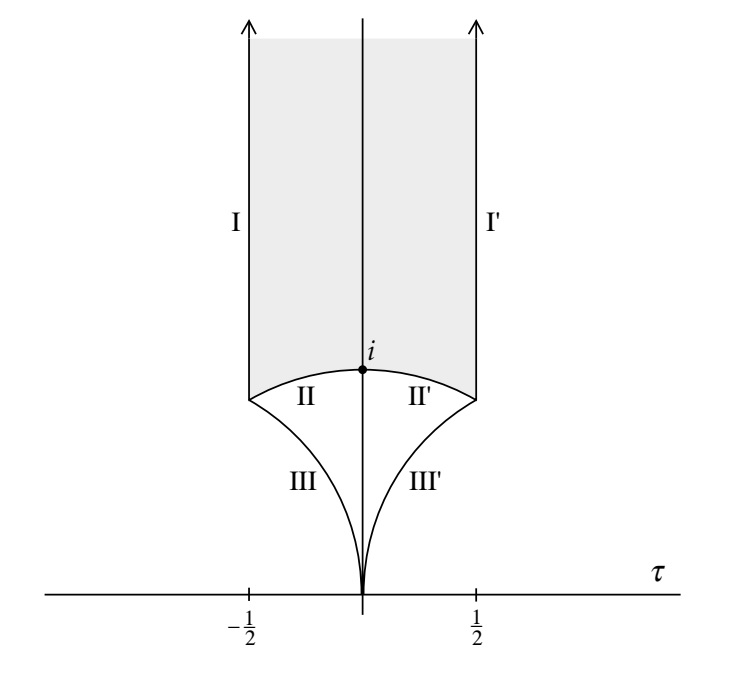
\includegraphics[width=0.5\textwidth,natwidth=546.75,natheight=504.75]{Fig5.2.jpg}\\
		\caption{The standard fundamental region $F_{0}$ for the moduli space of the torus, shaded. The lines I and I' are identified, as are the arcs II and II'. A different fundamental region, mapped into $F_{0}$ by the modular transformation $S$, is bounded by II, II', III, and III'.}\label{Fig5.2}
	\end{center}
\end{figure}

\begin{equation}
	-\frac{1}{2} \leq \operatorname{Re} \tau \leq \frac{1}{2}, \quad|\tau| \geq 1
\end{equation}
除了图中所示等价起来的边界,这被称为上半平面模掉 $\bmod P S L(2, \mathbf{Z})$的基本区域. 由于等价性,可以认为$F_{0}$ 被卷起来,仅当 $\operatorname{Im} \tau \rightarrow \infty$时开放. 基本区域 $F_{0}$ 是 ( diff $\times$ Weyl)不等价度规的模空间的一个表示.\\
对于点粒子有进一步的困难. 要求度规采取形式 (5.1.9) ,其中 $\tau$处在一个给定的基本区域,这并不固定所有的 diff $\times$ Weyl不变性. 度规以及周期性在刚性变换下不变
\begin{equation}
	\sigma^{a} \rightarrow \sigma^{a}+v^{a}
\end{equation}
所以该 diff $\times$ Weyl 二参量子群没有被固定. 另外,离散变换 $\sigma^{a} \rightarrow-\sigma^{a}$使度规不变,并且在非定向情况下$\tau \rightarrow-\bar{\tau}$的 $\left(\sigma^{1}, \sigma^{2}\right) \rightarrow\left(-\sigma^{1}, \sigma^{2}\right)$ 也使度规不变 . 因此这里又有了度规自由度与定域对称性之间的不匹配:度规中的参量不能被对称性移除,并且对称性没有被度规的选择所固定. 未固定的对称性称为共形Killing 群(C K G) .\\
当振幅中有足够多的顶点时,通过固定某些顶点算符的位置,我们可以完全固定规范不变性. 在有n个顶点算符的环面上,不变性(5.1.16) 可以用来固定一个顶点算符的位置,留下对$\tau$ 的积分,以及n-1个其他位置.  来自$\sigma^{a} \rightarrow-\sigma^{a}$ 的 $\mathbf{Z}_{2}$ 可以被要求第二个顶点算符在环面的中间固定 . 实际上,对于有限的重复计数,留下一些不固定的对称性,并除以一个合适的因子通常更方便些. 另外,如果顶点算符过少,某些共形Killing不变性仍然未固定,那么我们必须明确考虑重复计数.\\

\centerline{\Large 对读者的note}
在本章剩余部分,我们将更一般地讨论模. 主要目标是弦S矩阵的规范固定表达式 (5.3.9) . 事实上,大多数有趣的弦物理在树图振幅和一圈振幅就可以看到. 由于这个原因,测度可以通过捷径获得. 对于树图振幅,没有度规模但某些顶点算符的位置必须确定下来. 可以像(6.4.4)下面所阐述的那样推理出测度. 对于一圈振幅,通过类比(7.3.9)下面关于点粒子的讨论,可以以一种相对直观的方式理解测度. 

\section{模和Riemann面}%{5.2 Moduli and Riemann surfaces}

现在,我们以一种更普遍更抽象的方式重复之上的讨论. 我们以对某些给定拓扑 $r$上的所有度规积分. 称该度规空间为 $\mathscr{G}_{r} $ . 对于闭定向曲面,我们可以用柄的数目g,也称为亏格,来标记$r$ . 在考虑了diff $\times$ Weyl 冗余后,我们留下了模空间
\begin{equation}
	\mathscr{M}_{r}=\frac{\mathscr{G}_{r}}{(\text { diff } \times \mathrm{Weyl})_{r}}
\end{equation}
就像在环面情况那样,这个空间被有限个模参量化. 对于环面,$M_{1}$ 是上半平面模掉 $\bmod P S L(2, \mathbf{Z})$, 或等价地任意基本区域如 $F_{0}$. 还有可能存在diff $\times$ Weyl子群, 即 CKG, 使度规不变.\\
当在路径积分中有顶点算符时,用与度规中模的同等地位,看到它的位置是有用的. 当我们需要作出区分时,我们将指度规模. 一种处理CKG的方式,如果在路径积分中存在顶点算符时是适用的,是通过确定某些顶点算符的位置进一步指定规范. Polyakov路径积分包含对 $\mathscr{G}_{r}$ 的积分,以及n个顶点算符对世界面 $\mathscr{M} $的积分. 那么拓扑 $r$ 上有顶点算符的模空间是
\begin{equation}
	\mathscr{M}_{r, n}=\frac{\mathscr{G}_{r} \times M^{n}}{(\text { diff } \times \mathrm{Weyl})_{r}}
\end{equation}
就像我们在环面中看到的, $\operatorname{diff}_{r}$ 一般不是连通的. 选出包含单位元的连通部分 diff $_{r 0}$ ,商
\begin{equation}
	\frac{\operatorname{diff}_{r}}{\operatorname{diff}_{r 0}}
\end{equation}
是模群.\\
研究无限小层次上的度规的diff $\times$ Weyl冗余是很有趣的. 即,寻找一些不等价于diff $\times$ Weyl 变换的度规变分,因而等价于模中的改变. 我们也要寻找某些不改变度规的diff $\times$ Weyl 变换,这些是CKG的无限小元, 称为共形Killing矢量 ( $C K V s)$. \\
一个无限小的diff $\times$ Weyl变换对度规的改变为
\begin{equation}
	\delta g_{a b}=-2\left(P_{1} \delta \sigma\right)_{a b}+(2 \delta \omega-\nabla \cdot \delta \sigma) g_{a b}
\end{equation}
其中 $P_{1}$ 是导数的无迹对称线性组合 (3.3.17). 模所对应的度规变分 $\delta^{\prime} g_{a b}$与所有变分 (5.2 .4)正交 :
\begin{equation}
	\begin{aligned}
		0 &=\int d^{2} \sigma g^{1 / 2} \delta^{\prime} g_{a b}\left[-2\left(P_{1} \delta \sigma\right)^{a b}+(2 \delta \omega-\nabla \cdot \delta \sigma) g^{a b}\right] \\
		&=\int d^{2} \sigma g^{1 / 2}\left[-2\left(P_{1}^{T} \delta^{\prime} g\right)_{a} \delta \sigma^{a}+\delta^{\prime} g_{a b} g^{a b}(2 \delta \omega-\nabla \cdot \delta \sigma)\right]
	\end{aligned}
\end{equation}
其中平移 $\left(P_{1}^{T} u\right)_{a}=-\nabla^{b} u_{a b}$. \\

\fbox{\noindent\centering\parbox{0.9\textwidth}{注:\\
		$$
		\begin{aligned}
		(P, \delta \sigma)^{a b}&=\frac{1}{2}\left(\nabla^{a} \delta \sigma^{b}+\nabla^{b} \delta \sigma^{a}-g^{a b} \nabla \cdot \delta \sigma\right) \\
		\delta^{\prime} g_{a b}(P, \delta \sigma)^{a b}&=\frac{1}{2}\left(\delta^{\prime} g_{a b} \nabla^{a} \delta \sigma^{b}+\delta^{\prime} g_{a b} \nabla^{b} \delta \sigma^{a}-\delta^{\prime} g_{a b} g^{a b} \nabla \cdot \delta \sigma\right)
		\end{aligned}
		$$}}\\

为了使重叠(5.2 .5) 对于一般的$\delta \omega$ 与 $\delta \sigma$ 为零,我们需要
\begin{subequations}
\begin{equation}
g^{a b} \delta^{\prime} g_{a b} =0 
\end{equation}	
\begin{equation}
\left(P_{1}^{T} \delta^{\prime} g\right)_{a} =0
\end{equation}			
\end{subequations}
第一个条件要求 $\delta^{\prime} g_{a b}$ 无迹,并且是 $P_{1}^{T}$ 作用的无迹对称张量. 对于这些方程的每一解,都存在一个模.\\

CKVs 是使得 $\delta g_{a b}=0 $的(5.2 .4),该方程的迹唯一确定了 $\delta \omega$ , 留下了共形 Killing 方程
\begin{equation}
	\left(P_{1} \delta \sigma\right)_{a b}=0
\end{equation}
(5.2.6) 和 (5.2.7) 对共形规范周围的变分变得简单
\begin{subequations}
\begin{equation}
\partial_{\bar{z}} \delta^{\prime} g_{z z} =\partial_{z} \delta^{\prime} g_{\bar{z} \bar{z}}=0 
\end{equation}	
\begin{equation}
\partial_{\bar{z}} \delta z =\partial_{z} \delta \bar{z}=0
\end{equation}			
\end{subequations}
所以模的变分对应于全纯二次微分,而CKV对应全纯矢量场. 在环面上,唯一的全纯双周期函数是常数,所以存在两个实模以及两个实的CKV,与上节讨论一致.
度规模对应$P_{1}^{T}$的核(5.2 .6),而CKV对应$P_{1}$的核 (5.2 .7). Riemann-Roch定理将度规模数 $\mu=\operatorname{dim} \operatorname{ker} P_{1}^{T}$ 以及CKVs的数目$ \kappa=\operatorname{dim} \operatorname{ker} P_{1}$与Euler数 $\chi$相关联
\begin{equation}
	\mu-\kappa=-3 \chi
\end{equation}
我们将在本章后面推导它. 对于闭定向曲面 $-3 \chi=6 g-6 $ . 这个计数针对实模,将复数模例如 $\tau$ 分成了实部核虚部.
进一步,$\kappa$ 对于 $\chi<0$ 为零, $\mu$对 $\chi>0 $为零. 为证明这点,我们引用如下性质:总能通过Weyl变换找到一度规,其标量曲率 $R$ 为常数. 这样 $R$ 与 $\chi$符号相同. 现在, $P_{1}^{T} P_{1}=-\frac{1}{2} \nabla^{2}-\frac{1}{4} R$, 所以
\begin{equation}
	\begin{aligned}
		\int d^{2} \sigma g^{1 / 2}\left(P_{1} \delta \sigma\right)_{a b}\left(P_{1} \delta \sigma\right)^{a b} &=\int d^{2} \sigma g^{1 / 2} \delta \sigma_{a}\left(P_{1}^{T} P_{1} \delta \sigma\right)^{a} \\
		&=\int d^{2} \sigma g^{1 / 2}\left(\frac{1}{2} \nabla_{a} \delta \sigma_{b} \nabla^{a} \delta \sigma^{b}-\frac{R}{4} \delta \sigma_{a} \delta \sigma^{a}\right)
	\end{aligned}
\end{equation}
对于负的 $\chi$,右边是严格正定的,所以 $P_{1} \delta \sigma$ 不可能为零. 一个类似的讨论表明,对于正的 $\chi$, $P_{1}^{T} \delta^{\prime} g$不能为零. 结合这些结果,我们有
\begin{subequations}
\begin{equation}
\chi>0:  \kappa=3 \chi, \quad \mu=0 
\end{equation}
\begin{equation}
\chi<0:  \kappa=0, \quad \mu=-3 \chi
\end{equation}						
\end{subequations}

\centerline{\Large Riemann面}
描述模空间的常见方法是从每个等价类中选择一个度规,这构成依赖模$t^{k} $ 的度规族$\hat{g}_{a b}(t ; \sigma)$. 对于环面,(5.1.9) 给出这样一个切片. 使用(5.1.11)的另一描述通常比较方便, 其中 $d w d \bar{w}$ 被固定,而模被编码在坐标区域. 我们可以对这一概念进行如下形式化.\\
我们先来回忆可微流形是如何被定义的. 用一组相互交叠的集覆盖流形, $\sigma_{m}^{a}$ 是第 m个坐标卡中的坐标,而 $a$从 1取到流形的维数. 当坐标卡m与n交叠时,两个坐标卡中的坐标通过如下公式相关
\begin{equation}
	\sigma_{m}^{a}=f_{m n}^{a}\left(\sigma_{n}\right)
\end{equation}
其中要求传递函数能微分给定次. 对于 Riemannian流形,在每个坐标卡中同样给定了度规 $g_{m, a b}\left(\sigma_{m}\right)$ ,而重叠区的值通过通常的张量法则相关.\\
对于一个复流形,在每个坐标卡中存在复坐标 $z_{m}^{a}$ ,而现在a从1取到流形维数的一半. 传递函数被要求是全纯的
\begin{equation}
	z_{m}^{a}=f_{m n}^{a}\left(z_{n}\right)
\end{equation}
由于全纯性不依赖所使用的坐标 $z_{m}^{a}$. 现在可以定义流形上的全纯函数. 正如,如果两个可微流形之间存在一对一可微映射,它们就等价;如果两个复流形之间存在一对一全纯映射,它们就等价. 特别地,在每个坐标卡内做一个全纯的坐标变换,将给出等价的表面.\\
在二维情况 (一个复坐标), 复流形被称为Riemann面. 在这一情况下存在一一对应
\begin{equation}
\text{Riemann surfaces} \leftrightarrow \text{Riemannian manifolds mod Weyl}
\end{equation}
我们在右边放置了 'mod Weyl' 是因为 'mod diff' 已经隐含在 Riemannian 流形的定义中. 为了看到这个同构,从Riemannian 流形出发. 从我们对共形规范的讨论中,我们知道,可以在每个坐标卡中找到 $z_{m}$ 使得
\begin{equation}
	d s^{2} \propto d z_{m} d \bar{z}_{m}
\end{equation}
在临近的卡中,坐标不需要是相同的,但由于 $d s^{2} \propto d z_{m} d \bar{z}_{m} \propto d z_{n} d \bar{z}_{n}$, 传递函数是全纯的. 这是从Riemannian manifolds到两实维的复流形的映射. 对于逆映射,可以在第m个卡中取度规 $d z_{m} d \bar{z}_{m}$,并使其在交叠区光滑以产生Riemannian 流形. Riemann面的两个表征因而是等价的.\\
以平行四边形 (\ref{Fig5.1}) 的复坐标w来描述环面例证了复流形的思想. 假想取单个坐标卡,其比(\ref{Fig5.1}) 的基本平行四边形大一点. 那么,周期性条件
\begin{equation}
	w \cong w+2 \pi \cong w+2 \pi \tau
\end{equation}
就是坐标卡两个相反边缘的交叠上的传递函数. 这些传递函数定义了面. 为了定义原始的对度规的路径积分,将度规视为固定坐标,例如平方 (5.1.7), 或至少是传递函数固定的坐标卡的固定集合,是最简单的出发点. 为了研究给定平面上的量子场论,那么最简单的就是处理传递函数模相关的单位度规,就像平行四边形(5.1.11)中那样.\\
也可以如下看到Rieman面. 定义世界面为坐标卡的并. 我们可以用 diff $\times$ Weyl 自由度在每一坐标卡中达到度规 $d z d \bar{z}$.这样在坐标卡交叠区的规范选择只能相差该度规的diff $\times$ Weyl 不变. 这正是我们讨论过的共形变换. 因而Rieman面是CFT自然生长的地方,这是因为CFT中的场在共形变换下有明确的变换性质.

\section{模的测度}%{5.3 The measure for moduli}
我们现在回顾Polyakov路径积分的规范固定.  我们已经知道了规范冗余不完全消除对度规的路径积分,但留下了模空间上的有限维积分. 为了将其考虑在内,有必要精炼3.3节的讨论.\\
S矩阵的路径积分是
\begin{equation}
	\begin{aligned}
		&S_{j_{1} \ldots j_{n}}\left(k_{1}, \ldots, k_{n}\right) \\
		&\quad=\sum_{\begin{array}{l}
				\text { compact } \\
				\text { topologies }
		\end{array}} \int \frac{[d \phi d g]}{V_{\text {diff }} \times \text { Weyl }} \exp \left(-S_{\mathrm{m}}-\lambda \chi\right) \prod_{i=1}^{n} \int d^{2} \sigma_{i} g\left(\sigma_{i}\right)^{1 / 2} \mathscr{V}_{j_{i}}\left(k_{i}, \sigma_{i}\right)
	\end{aligned}
\end{equation}
这是之前的表达式(3.5.5) ,但现在有一个$c=\tilde{c}=26$ 的普遍物质场,物质场用 $\phi $标记. 在规范固定中,对度规和位置的积分换成对规范群、模以及未定位置的积分
\begin{equation}
	[d g] d^{2 n} \sigma \rightarrow[d \zeta] d^{\mu} t d^{2 n-\kappa} \sigma
\end{equation}
在因式分解出规范体积后,这一变换的Jacobian行列式就变成了模空间上的测度.\\
这一步与3.3节是相同的,现在将模与CKV考虑在内.特别地,规范选择现在会固定 $\kappa$ 个顶点坐标, $\sigma_{i}^{a} \rightarrow \hat{\sigma}_{i}^{a} $ . 记固定坐标 $(a, i)$ 的集合为 $f $ ,定义模空间上的Faddeev-Popov测度为
\begin{equation}
	1=\Delta_{\mathrm{FP}}(g, \sigma) \int_{F} d^{\mu} t \int_{\mathrm{diff} \times \mathrm{Weyl}}[d \zeta] \delta\left(g-\hat{g}(t)^{\zeta}\right) \prod_{(a, i) \in f} \delta\left(\sigma_{i}^{a}-\hat{\sigma}_{i}^{\zeta a}\right)
\end{equation}
通过定义,每个度规 (diff $\times$ Weyl)等价于一个$t$ and $\zeta $的$\hat{g}(t)$ . 实际上,正如5.1节末尾所讨论的,可能会存在一个残留的有限阶 $n_{R}$的离散对称群,所以delta函数在$n_{R}$个点非零.\\
将(5.3.3) 代入路径积分 (5.3.1) ,并使用与之前相同步骤给出
\begin{equation}
	\begin{aligned}
		S_{j_{1} \ldots j_{n}}\left(k_{1}, \ldots, k_{n}\right)=& \sum_{\text {compact },\text { topologies } } \int_{F} d^{\mu} t \Delta_{\mathrm{FP}}(\hat{g}(t), \hat{\sigma}) \int[d \phi] \int \prod_{(a, i) \notin f} d \sigma_{i}^{a} \\	
		&\times \exp \left(-S_{\mathrm{m}}[\phi, \hat{g}(t)]-\lambda \chi\right) \prod_{i=1}^{n}\left[\hat{g}\left(\sigma_{i}\right)^{1 / 2} \mathscr{N}_{j_{i}}\left(k_{i} ; \sigma_{i}\right)\right]
	\end{aligned}
\end{equation}
对度规和顶点算符坐标的积分现在退化成对度规和未定坐标的模空间 $F$加上 $\Delta_{\mathrm{FP}} $ 给定的测度的积分. 在顶点算符中,$\kappa$个位置被固定了.\\
现在我们计算Faddeev-Popov测度. delta函数在对称相关的 $n_{R}$个点上非零,所以我们考察一个这样的点并除以$n_{R} $ . 在该点附近展开$\Delta_{\mathrm{FP}}$的定义(5.3 .3). 一般度规变分等于定域对称变分加上模 $t^{k}$的一个变化,
\begin{equation}
	\delta g_{a b}=\sum_{k=1}^{\mu} \delta t^{k} \partial_{t^{k}} \hat{g}_{a b}-2\left(\hat{P}_{1} \delta \sigma\right)_{a b}+(2 \delta \omega-\hat{\nabla} \cdot \delta \sigma) \hat{g}_{a b}
\end{equation}
Faddeev-Popov逆行列式为
\begin{equation}
	\begin{aligned}
		&\Delta_{\mathrm{FP}}(\hat{g}, \hat{\sigma})^{-1} \\
		&=n_{R} \int d^{\mu} \delta t[d \delta \omega d \delta \sigma] \delta\left(\delta g_{a b}\right) \prod_{(a, i) \in f} \delta\left(\delta \sigma^{a}\left(\hat{\sigma}_{i}\right)\right)\\
		&=n_{R}  \int d^{\mu} \delta t d^{\kappa} x\left[d \beta^{\prime} d \delta \sigma\right] \\
		&\quad \times \exp \left[2 \pi i\left(\beta^{\prime}, 2 \hat{P}_{1} \delta \sigma-\delta t^{k} \partial_{k} \hat{g}\right)+2 \pi i \sum_{(a, i) \in f} x_{a i} \delta \sigma^{a}\left(\hat{\sigma}_{i}\right)\right]
	\end{aligned}
\end{equation}
第二行中内积的定义参考习题3.2. 我们跟随了与3.3节相同的定域讨论,将delta函数与泛函写成对$x$ 与 $\beta_{a b}$ 的积分,并积掉 $\delta \omega$ 以获得 $\beta_{a b}^{\prime}$ 是无迹的约束.\\
像之前一样,将所有bosonic变量替换成Grassmann变量来转换积分(5.3 .6):
\begin{subequations}
\begin{equation}
\delta \sigma^{a}  \rightarrow c^{a} 
\end{equation}
\begin{equation}
\beta_{a b}^{\prime}  \rightarrow b_{a b} 
\end{equation}
\begin{equation}
x_{a i}  \rightarrow \eta_{a i} 
\end{equation}
\begin{equation}
\delta t^{k}  \rightarrow \xi^{k}
\end{equation}	
\end{subequations}
然后,在场的传统归一化下
\begin{equation}
	\begin{aligned}
		\Delta_{\mathrm{FP}}(\hat{\mathrm{g}}, \hat{\sigma})=& \frac{1}{n_{R}} \int[d b d c] d^{\mu} \xi d^{\kappa} \eta \\
		&\quad \times \exp \left[-\frac{1}{4 \pi}\left(b, 2 \hat{P}_{1} c-\xi^{k} \partial_{k} \hat{g}\right)+\sum_{(a, i) \in f} \eta_{a i} c^{a}\left(\hat{\sigma}_{i}\right)\right] \\
		=& \frac{1}{n_{R}} \int[d b d c] \exp \left(-S_{\mathrm{g}}\right) \prod_{k=1}^{\mu} \frac{1}{4 \pi}\left(b, \partial_{k} \hat{g}\right) \prod_{(a, i) \in f} c^{a}\left(\hat{\sigma}_{i}\right)
	\end{aligned}
\end{equation}
在最后一行,我们积掉了Grassmann 变量 $\eta_{a i}$和 $\xi^{k}$.\\
模空间上合适的积分测度由带有该插入鬼路径积分生成. 我们不试图在中间步骤保留总符号的踪迹;既然这是一个Jacobian行列式,我们可以暗中选择总符号以给出正的结果. S矩阵的完整表达式是
\begin{equation}
	\begin{aligned}
		&S_{j_{1} \ldots j_{n}}\left(k_{1}, \ldots, k_{n}\right)\\
		&=\sum_{\text {compact },\text { topologies }} \int_{F} \frac{d^{\mu} t}{n_{R}} \int[d \phi d b d c] \exp \left(-S_{\mathrm{m}}-S_{\mathrm{g}}-\lambda \chi\right) \\
		&\times \prod_{(a, i) \notin f} \int d \sigma_{i}^{a} \prod_{k=1}^{\mu} \frac{1}{4 \pi}\left(b, \partial_{k} \hat{g}\right) \prod_{(a, i) \in f} c^{a}\left(\hat{\sigma}_{i}\right) \prod_{i=1}^{n} \hat{g}\left(\sigma_{i}\right)^{1 / 2} \mathscr{V}_{j_{i}}\left(k_{i}, \sigma_{i}\right)
	\end{aligned}
\end{equation}
这一结果随时可以扩展到所有bosonic弦理论 - 闭的或开的,定向或非定向的-唯一的差异是要纳入什么样的拓扑并允许什么样的顶点算符. Eq. (5.3.9) 是一个有用且漂亮的结果. 模和CKV引入的复杂性通过在路径积分中插入b和c而考虑在内. 对于每个固定坐标, $d \sigma_{i}^{a}$被替换成 $c_{i}^{a}$, 而每个度规模给出b插入.

\centerline{\Large 行列式形式的表示}
在 (5.3.8) 中,我们将Faddeev-Popov行列式表示成对Grassmann变量和场的积分.我们现在要将其化简成有限维泛函行列式的乘积. 当我们在接下来的章节中继续研究弦S矩阵时,这一直接的路径积分方法仅是我们要使用的方法之一.\\
在合适的完备基下展开鬼场
\begin{equation}
	c^{a}(\sigma)=\sum_{J} c_{J} \mathrm{C}_{J}^{a}(\sigma), \quad b_{a b}(\sigma)=\sum_{K} b_{K} \mathrm{~B}_{K a b}(\sigma)
\end{equation}
完备基 $C_{J}^{a}$ 与 $B_{K a b}$定义如下. 出现在鬼作用量中的导数 $P_{1}$ 将矢量转换成无迹对称张量. 而它的转置是相反的功能. 鬼作用量可以写成
\begin{equation}
	S_{\mathrm{g}}=\frac{1}{2 \pi}\left(b, P_{1} c\right)=\frac{1}{2 \pi}\left(P_{1}^{T} b, c\right)
\end{equation}
我们无法以一种diff不变的方式对角化 $P_{1}$,因为它将一种场转化成另一种,但我们可以对角化$P_{1}^{T} P_{1}$ 和 $P_{1} P_{1}^{T}$:
\begin{equation}
	P_{1}^{T} P_{1} \mathrm{C}_{J}^{a}=v_{J}^{\prime 2} \mathrm{C}_{J}^{a}, \quad P_{1} P_{1}^{T} \mathrm{~B}_{K a b}=v_{K}^{2} \mathrm{~B}_{K a b}
\end{equation}
本征函数可以选为实的,并在如下内积中归一化
\begin{subequations}
\begin{equation}
\left(\mathrm{C}_{J}, \mathrm{C}_{J^{\prime}}\right) =\int d^{2} \sigma g^{1 / 2} \mathrm{C}_{J}^{a} \mathrm{C}_{J^{\prime} a}=\delta_{J J^{\prime}} 
\end{equation}
\begin{equation}
\left(\mathrm{B}_{K}, \mathrm{~B}_{K^{\prime}}\right) =\int d^{2} \sigma g^{1 / 2} \mathrm{~B}_{K a b} \mathrm{~B}_{K^{\prime}}^{a b}=\delta_{K K^{\prime}}
\end{equation}
\end{subequations}
现在注意到
\begin{equation}
	\left(P_{1} P_{1}^{T}\right) P_{1} \mathrm{C}_{J}=P_{1}\left(P_{1}^{T} P_{1}\right) \mathrm{C}_{J}=v_{J}^{\prime 2} P_{1} \mathrm{C}_{J}
\end{equation}
所以 $P_{1} \mathrm{C}_{J}$是 $P_{1} P_{1}^{T} $的本征函数. 以同样方法, $P_{1}^{T} \mathrm{~B}_{K}$ 是 $P_{1}^{T} P_{1} $的本征函数. 因此除了 $P_{1} \mathrm{C}_{J}=0$ 或 $P_{1}^{T} \mathrm{~B}_{K}=0 $,本征函数之间存在一一映射.  它们对应 $P_{1}^{T} P_{1}$ 或 $P_{1} P_{1}^{T} $的本征值. 它们正是CKV和全纯二次微分,因而它们的数目分别是 $\kappa$ 和 $\mu$. 我们将零本征值的本征函数记为 $\mathrm{C}_{0 j}$ 或$\mathrm{B}_{0 k}$, 而非零本征值被标记为 $J, K=1, \ldots$ . 对于后者,归一化关联函数的关联为
\begin{equation}
	\mathrm{B}_{J a b}=\frac{1}{v_{J}}\left(P_{1} \mathrm{C}_{J}\right)_{a b}, \quad v_{J}=v_{J}^{\prime} \neq 0
\end{equation}
以模的形式,鬼路径积分 $\Delta_{\mathrm{FP}}$ 变成
\begin{equation}
	\int \prod_{k=1}^{\mu} d b_{0 k} \prod_{j=1}^{\kappa} d c_{0 j} \prod_{J} d b_{J} d c_{J} \exp \left(-\frac{v_{J} b_{J} c_{J}}{2 \pi}\right) \prod_{k^{\prime}=1}^{\mu} \frac{1}{4 \pi}\left(b, \partial_{k^{\prime}} \hat{g}\right) \prod_{(a, i) \in f} c^{a}\left(\sigma_{i}\right)
\end{equation}
从A.2节,我们知道,除非变量出现在被积函数中,否则Grassmann积分为零. $c_{0 j}$ 和 $b_{0 k}$ 没有出现在作用量中,而仅仅出现在插入中. 事实上,积分(5.3 .16)中每一种插入的数目,$ \kappa$ 和 $\mu$ ,分别与鬼零模匹配. 我们恰好有足够多的插入以给出非零的结果,并且在插入中,只有鬼场的零模部分有贡献. 因此
\begin{equation}
	\begin{aligned}
		\Delta_{\mathrm{FP}}=\int \prod_{k=1}^{\mu} & d b_{0 k} \prod_{k^{\prime}=1}^{\mu}\left[\sum_{k^{\prime \prime}=1}^{\mu} \frac{b_{0 k^{\prime \prime}}}{4 \pi}\left(\mathrm{B}_{0 k^{\prime \prime}}, \partial_{k^{\prime}} \hat{g}\right)\right] \\
		& \times \int \prod_{j=1}^{\kappa} d c_{0 j} \prod_{(a, i) \in f}\left[\sum_{j^{\prime}=1}^{\kappa} c_{0 j^{\prime}} \mathrm{C}_{0 j^{\prime}}^{a}\left(\sigma_{i}\right)\right] \\
		& \times \int \prod_{J} d b_{J} d c_{J} \exp \left(-\frac{v_{J} b_{J} c_{J}}{2 \pi}\right)
	\end{aligned}
\end{equation}
对所有使得零模积分充满Grassmann变量的方式求和,在每种情况下,积分会生成有限行列式,而非零模产生一个无穷乘积,一个泛函行列式. 合起来
\begin{equation}
	\Delta_{\mathrm{FP}}=\operatorname{det} \frac{\left(\mathrm{B}_{0 k}, \partial_{k^{\prime}} \hat{g}\right)}{4 \pi} \operatorname{det} C_{0 j}^{a}\left(\sigma_{i}\right) \operatorname{det}^{\prime}\left(\frac{P_{1}^{T} P_{1}}{4 \pi^{2}}\right)^{1 / 2}
\end{equation}
注意到$\mathrm{C}_{0 j}^{a}\left(\sigma_{i}\right)$ 是平方矩阵,其中 $(a, i) \in f$ 像j一样取遍 $\kappa$ 个值.泛函行列式上的撇代表去掉了零本征值.\\

\centerline{\Large Riemann- Roch定理}
我们现在给出Riemann-Roch 定理的一个路径积分推导.对于全纯 $b c$ 系统 (没有 $\tilde{b}, \tilde{c}$)的鬼流, 习题3.6中导出的流守恒反常是
\begin{equation}
	\nabla_{a} j^{a}=\frac{1-2 \lambda}{4} R
\end{equation}
Noether定理将流守恒与不变性相关联. 对于不守恒流,通过讨论发现
\begin{equation}
	\frac{\delta([d \phi] \exp (-S))}{[d \phi] \exp (-S)}=\frac{i \epsilon}{2 \pi} \int d^{2} \sigma g^{1 / 2} \nabla_{a} j^{a} \rightarrow-i \epsilon \frac{2 \lambda-1}{2} \chi
\end{equation}
鬼数对称性的作用为 $\delta b=-i \epsilon b, \delta c=i \epsilon c $.  当路径积分非零时,测度、作用量和插入的变换必须相互抵消. 因此,从反常中我们了解到c插入的数目减去b插入的数目是$3 \chi / 2 $.  路径积分计算将插入的数目与零模的数目关联起来,因而给出相同的差值
\begin{equation}
	\frac{1}{2}(\kappa-\mu)=\frac{1}{2}\left(\operatorname{dim} \operatorname{ker} P_{1}-\operatorname{dim} \operatorname{ker} P_{1}^{T}\right)
\end{equation}
因子 $\frac{1}{2}$的出现是因为我们仅仅取出了全纯理论,反全纯理论给出相同贡献. 等同从反常中得到的结果与从零模中得到的结果给出Riemann-Roch 定理 $\kappa-\mu=3 \chi$. 对一般的$b c$系统,以相同方式会发现
\begin{equation}
	\operatorname{dim} \operatorname{ker} P_{n}-\operatorname{dim} \operatorname{ker} P_{n}^{T}=(2 n+1) \chi
\end{equation}
$P_{n}$算符在习题3.2中定义.

\section{关于测度的更多介绍}%{5.4 More about the measure}
这里我们收集了一些规范固定弦振幅的普遍性质. 它们对于第9章中的更加形式化的考察由奠基性的作用.\\

\centerline{\Large 规范不变性}
Faddeev-Popov处理所生成的规范固定振幅是BRST不变且独立于规范选择. 然而,明确的检验它是否有期望的全部性质是很有用的. \\
第一,它独立于模空间上坐标t的选择. 对于新坐标$t^{\prime k}(t)$
\begin{equation}
	\begin{aligned}
		d^{\mu} t^{\prime} &=\left|\operatorname{det} \frac{\partial t^{\prime}}{\partial t}\right| d^{\mu} t \\
		\prod_{k=1}^{\mu} \frac{1}{4 \pi}\left(b, \partial_{k}^{\prime} \hat{g}\right) &=\operatorname{det}\left(\frac{\partial t}{\partial t^{\prime}}\right) \prod_{k=1}^{\mu} \frac{1}{4 \pi}\left(b, \partial_{k} \hat{g}\right)
	\end{aligned}
\end{equation}
并且这两个Jacobians行列式相互抵消 (相差一个符号,我们会手动决定以给出一个正的测度). 换句话说,b鬼引起的积分像模空间上的密度那样变换.\\
第二,我们来看一下该测度在规范切片的Weyl变换下不变. 在Weyl变换下,
\begin{equation}
	\delta \hat{g}_{a b}^{\prime}(t ; \sigma)=2 \delta \omega(t ; \sigma) \hat{g}_{a b}(t ; \sigma)
\end{equation}
作用量和测度的变分给出了定域算符$T_{a}^{a}$的插入,其在 $D=26$ 由于运动方程而为零. 因而,我们只需要关心各个插入上的效应. 顶点算符插入由于收缩进而为零.插入 $c^{a}\left(\sigma_{i}\right)$ 根据 (3.3.24)下面的讨论而为零. 对于
\begin{equation}
	\begin{aligned}
		\left(b, \partial_{k} \hat{g}^{\prime}\right) &=\int d^{2} \sigma \hat{g}^{\prime 1 / 2} b_{a b} \hat{g}^{\prime a c} \hat{g}^{b d} \partial_{k} \hat{g}_{c d}^{\prime} \\
		&=\int d^{2} \sigma \hat{g}^{1 / 2} b_{a b}\left(\hat{g}^{a c} \hat{g}^{b d} \partial_{k} \hat{g}_{c d}+2 \hat{g}^{a b} \partial_{k} \omega\right) \\
		&=\left(b, \partial_{k} \hat{g}\right)
	\end{aligned}
\end{equation}
最后一个等式由于 $b$的无迹而成立.\\
第三,我们来检验无限小diff变换 $\delta \sigma=\xi(t ; \sigma) $下的不变性.  扩展到一般diff变换是直接的. 振幅(5.3.9)中唯一一个不是立即不变的项是b插入以及坐标被固定的顶点算符. 前者变换为
\begin{equation}
	\begin{aligned}
		\delta\left(b, \partial_{k} \hat{g}\right) &=-2\left(b, P_{1} \partial_{k} \xi\right) \\
		&=-2\left(P_{1}^{T} b, \partial_{k} \xi\right) \\
		&=0
	\end{aligned}
\end{equation}
其中利用了b的运动方程. b运动方程来自$\delta S / \delta c=0$,所以在c插入上会存在源项; 它们是解释坐标变换在固定顶点算符上的效应所需要的.\\

\centerline{\Large BRST不变性}
我们现在来证明(5.3 .9)的全BRST不变性 . 从定域分析中知道路径积分测度与作用量是不变的,所以我们不得不考察BRST变换在插入上的效应. 在规范固定路径积分(5.3.9)中,非定向顶点算符伴随着因子 $c$ 或 $\tilde{c} c$. 这是我们在4.4节末尾对对应于OCQ态的BRST不变顶点算符的描述. 另一方面,被积顶点算符不是BRST不变的,它们有BRST性质:
\begin{equation}
	\delta_{\mathrm{B}} \mathscr{V}_{\mathrm{m}}=i \epsilon \partial_{a}\left(c^{a} \mathscr{V}_{\mathrm{m}}\right)
\end{equation}
其在积分意义下为零.最终还有b插入的变分
\begin{equation}
	\delta_{\mathrm{B}}\left(b, \partial_{k} \hat{g}\right)=i \epsilon\left(T, \partial_{k} \hat{g}\right)
\end{equation}
能动量张量的插入仅产生了对$t^{k}$的导数,所以除了一个可能来自于模空间边界的项,BRST变分为零. 在下一章巡航,我们将检验模空间的边界. 在大多数情况不存在表面贡献,这是由于所谓的抵消传播子讨论. 在一定情形下,这个讨论并不适用,我们将看到如何处理这一点.\\
重要的是,规范固定结果(5.3 .9)可以直接从BRST不变性的要求写出来,而不用参考规范固定形式.正如我们在计算路径积分时候看到的,至少存在 $\mu $ 个b插入和 $\kappa $ 个c插入,否则路径积分为零. 在振幅(5.3.9)中正好存在数目正确的鬼插入以给出非零结果. 一旦我们引入必需的b因子,BRST变换在能动张量中带来与度规的$t^{k}$ 导数的卷积. 这正比于对模的导数,所以我们就像以前做的那样,对模空间积分就得到了一个不变的结果. 结果(5.3 .9)可以以各种方式推广. (例如共形Killing不变情况是保持不固定). 在第7章,对于无顶点算符的环面,我们将明确地例证这一点.BRST不变性暗示了BRST等价态的振幅是相同的. 如果我们给任意一个态增加一个空部分$Q_{B}|\chi\rangle$,效果是在路径积分中插入变分 $\delta_{B} \mathscr{V}_{\chi} $ ;这个积分为零. 这是重要的,因为物理Hilbert空间等同为上同调,所以等价态应该有相同振幅.\\

\centerline{\Large Riemann面的测度}
我们在规范固定世界面是由模-相关度规导出的框架中推导出了Faddeev-Popov测度.我们现在在Riemann面的框架中重铸这个结果,在这个框架中,结构被编码进入模相关传递函数中.\\
为了表示该测度在模空间中给定点$t_{0}$ 处的值,我们取一组坐标卡,在第m坐标卡有复坐标 $z_{m}$,以及全纯的传递函数,其中度规 $\hat{g}\left(t_{0}\right)$ 在每个坐标卡中等价于$d z_{m} d \bar{z}_{m}$ . 现在考察模的变化. 我们先将其描述为传递函数固定的度规中的变换,然后将其转化为度规固定的传递函数的变化. 在第一种描述中,定义Beltrami微分
\begin{equation}
	\mu_{k a}^{b}=\frac{1}{2} \hat{g}^{b c} \partial_{k} \hat{g}_{a c}
\end{equation}
 $\delta t^{k}$ 的b插入变成
\begin{equation}
	\frac{1}{2 \pi}\left(b, \mu_{k}\right)=\frac{1}{2 \pi} \int d^{2} z\left(b_{z z} \mu_{k \bar{z}}^{z}+b_{\bar{z} \bar{z}} \mu_{k z}^{\bar{z}}\right)
\end{equation}
在第二种描述中,在模中的变换 $\delta t^{k}$ 之后,在每个坐标卡中将会有新坐标
\begin{equation}
	z_{m}^{\prime}=z_{m}+\delta t^{k} v_{k m}^{z_{m}}\left(z_{m}, \bar{z}_{m}\right)
\end{equation}
$v_{k m}^{a}$ 上的上标是顶点指标;注意到 $v_{k m}^{a}$仅定义在第m个坐标卡中. 通过 Riemann 面的定义, $d z_{m}^{\prime} d \bar{z}_{m}^{\prime}$ 等价于 $t_{0}+\delta t$处的度规
\begin{equation}
	d z_{m}^{\prime} d \bar{z}_{m}^{\prime} \propto d z_{m} d \bar{z}_{m}+\delta t^{k}\left(\mu_{k z_{m}}^{\bar{z}_{m}} d z_{m} d z_{m}+\mu_{k \bar{z}_{m}}^{z_{m}} d \bar{z}_{m} d \bar{z}_{m}\right)
\end{equation}
因此坐标变化 $v_{k m}^{a}$与Beltrami微分的关系为
\begin{equation}
	\mu_{k z_{m}}^{\overline{\bar{z}}_{m}}=\partial_{z_{m}} v_{k m}^{\bar{z}_{m}}, \quad \mu_{k \bar{z}_{m}}^{z_{m}}=\partial_{\bar{z}_{m}} v_{k m}^{z_{m}}
\end{equation}
这是Beltrami方程的无穷小版本. 它暗示了$v_{k m}^{z_{m}}$ 不是全纯的,否则它将不对应模的变化.另外, $v_{k m}^{z_{m}}$ 中有一个不由Beltrami方程决定的全纯部分,对于 $v_{k m}^{\bar{z}_{m}}$则是反全纯部分;这些对应于每个坐标卡中做全纯再参量化的自由度.\\
分部积分,b插入 (5.4 .8)变成
\begin{equation}
	\frac{1}{2 \pi}\left(b, \mu_{k}\right)=\frac{1}{2 \pi i} \sum_{m} \oint_{C_{m}}\left(d z_{m} v_{k m}^{z_{m}} b_{z_{m} z_{m}}-d \bar{z}_{m} v_{k m}^{\bar{z}_{m}} b_{\bar{z}_{m} \bar{z}_{m}}\right)
\end{equation}
围道 $C_{m}$ 逆时针围绕第m个坐标卡. 通过(5.4.9),坐标对模的导数在给定点是
\begin{equation}
	\frac{d z_{m}}{d t^{k}}=v_{k m}^{z_{m}}
\end{equation}
因此,传递函数在模变换下的变换是
\begin{equation}
	\left.\frac{\partial z_{m}}{\partial t^{k}}\right|_{z_{n}}=v_{k m}^{z_{m}}-\frac{\partial z_{m}}{\partial z_{n}} \mid v_{t}^{z_{k n}}=v_{k m}^{z_{m}}-v_{k n}^{z_{m}}
\end{equation}
那么,结合环绕邻近坐标卡的围道积分 (5.4.12)给出
\begin{equation}
	\frac{1}{2 \pi}\left(b, \mu_{k}\right)=\frac{1}{2 \pi i} \sum_{(m n)} \int_{C_{m n}}\left(\left.d z_{m} \frac{\partial z_{m}}{\partial t^{k}}\right|_{z_{n}} b_{z_{m} z_{m}}-\left.d \bar{z}_{m} \frac{\partial \bar{z}_{m}}{\partial t^{k}}\right|_{z_{n}} b_{\bar{z}_{m} \bar{z}_{m}}\right)
\end{equation}
这正比于传递函数的导数. 求和取遍所有重叠的坐标卡. 围道 $C_{m n}$ 在卡$m$ 和 $n$之间跑动, 并在方向在$m$的视角下是逆时针的.   $(m n)$ 项关于 $m$ 和 $n$对称,但这并不显然. 每个围道要么闭合,要么在坐标卡 $m, n$和 $p$重合区域截止,在这里围道 $C_{m n}, C_{n p}$和$C_{p m}$ 交于一点.b插入现在以定义Riemann面的数据显式地表述出来,传递函数模掉了全纯等价性.\\
作为一个例证,我们可以用其将度规的模与顶点算符位置的模放在一个更加平等的基础上. 考察坐标系z中处于$z_{v}$ 处的顶点算符. 以顶点算符为中心做一个较小的新坐标卡 $z^{\prime}$, 如图(\ref{Fig5.3})所示. 

\begin{figure}
	\begin{center}
		%width=0.8\textwidth,bb=0 0 436 415
		%1px=0.75pt
		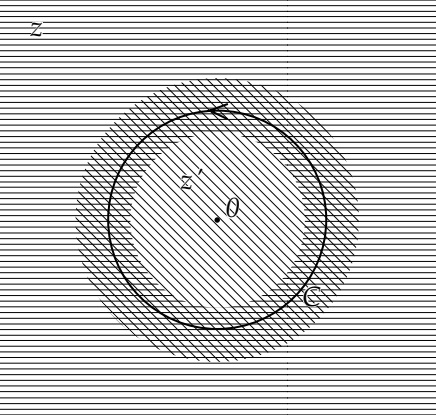
\includegraphics[width=0.5\textwidth,natwidth=327,natheight=311]{Fig5.3.jpg}\\
		\caption{Coordinate patches $z^{\prime}$ (diagonal hatching) and $z$ (horizontal hatching) with vertex operator at $z^{\prime}=0$. In the annular region, $z=z^{\prime}+z_{v}$.}\label{Fig5.3}
	\end{center}
\end{figure}

我们保留$z^{\prime}=0$处的顶点算符, 并将它的位置编码进传递函数中
\begin{equation}
	z=z^{\prime}+z_{v}
\end{equation}
 $z_{v}, \bar{z}_{v}$ 的测度由(5.4 .15)给定,其中
\begin{equation}
	\left.\frac{\partial z^{\prime}}{\partial z_{v}}\right|_{z}=-1
\end{equation}
因此,鬼插入是
\begin{equation}
	\int_{C} \frac{d z^{\prime}}{2 \pi i} b_{z^{\prime} z^{\prime}} \int_{C} \frac{d \bar{z}_{m}^{\prime}}{-2 \pi i} b_{\bar{z}^{\prime} \bar{z}^{\prime}}=b_{-1} \tilde{b}_{-1} \cdot
\end{equation}
其中 $C$ 是如图所示环绕顶点算符的任意围道.那么,S矩阵的完整表达式可以紧凑的写成
\begin{equation}
	S(1 ; \ldots ; n)=\sum_{\begin{array}{c}
			\text { compact } \atop \text { topologies }
	\end{array}} e^{-\lambda \chi} \int_{F} \frac{d^{m} t}{n_{R}}\left\langle\prod_{k=1}^{m} B_{k} \prod_{i=1}^{n} \hat{\mathscr{V}}_{i}\right\rangle
\end{equation}
这里, $B_{k}$ 是b鬼插入 (5.4 .15)的简写,而$\hat{\hat{V}}$ 对于闭弦代表 $\tilde{c} c \mathscr{K}_{\mathrm{m}}$,对于开弦代表 $t_{a} c^{a} \mathscr{\psi}_{\mathrm{m}}$. 即,我们现在将所有的顶点算符处理成固定的,并将它们的坐标换成传递函数中的额外参量.模的数目m是
\begin{equation}
	m=\mu+2 n_{\mathrm{c}}+n_{\mathrm{o}}-\kappa=-3 \chi+2 n_{\mathrm{c}}+n_{\mathrm{o}}
\end{equation}
其中 $n_{\mathrm{c}}$ 和 $n_{\mathrm{o}}$ 分别是闭弦顶点算符和开弦顶点算符的数目.\\
(5.4.19) 表明了戴帽的顶点算符,即含有 $\tilde{c} c$ 或 $t_{a} c^{a}$, 的算符是基础的. 这正是态-算符对应所产生的,并且它是BRST不变的. 如果顶点算符被积分了,鬼插入(5.4.18) 会移除$\tilde{c} c$或 $t_{a} c^{a} $ . 例如
\begin{equation}
	b_{-1} \tilde{b}_{-1} \cdot \tilde{c} c \mathscr{V}_{\mathrm{m}}=\mathscr{V}_{\mathrm{m}}
\end{equation}
留下了顶点算符的积分形式. 我们从Polyakov路径积分中写出 (5.4.19),所以顶点算符以OCQ的形式出现,但现在我们可以使用任意的BRST不变顶点算符.

